The ROUGE-Based Model is a simple \glsdisp{nn}{Neural Network} utilizing \gls{rouge} scores as its inputs. It was designed to predict the content score based on the summary and the reference text. While it does also predict the wording score, it does not perform as well on it.\\
The inspiration for this model arose during the exploration of existing methods for text evaluation. Among other metrics, such as \gls{bleu}, \gls{meteor} and \gls{perplexity}, \gls{rouge} stood out, as it was originally designed for assessing summaries.
However, as quoted in
\hyperref[sec:rouge_theory]{Chapter \ref{sec:rouge_theory}},
the \gls{rouge} Measures compare a computer-generated summary to a human-written one. So, for this project, it was adapted by substituting the machine-written summary with that of a student and replacing the (ideal) human-written summary with the full reference text.\\
\subsubsection{Model Architecture}
The ROUGE-Based Model consists of two distinct steps: the calculation of \gls{rouge}-scores and the forward pass through the neural network, as illustrated in
\hyperref[fig:rouge-based-model]{Figure~\ref{fig:rouge-based-model}}.
The \gls{rouge}-scores are computed from the \glsdisp{token}{tokenized} reference text and summary, after their stopwords were removed. The Precision, Recall, and F1-Score from the ROUGE-scores, along with the normalized length of the summary, serve as inputs to the network. The network then outputs the predicted content and wording scores for the summary.
\begin{figure}[H]
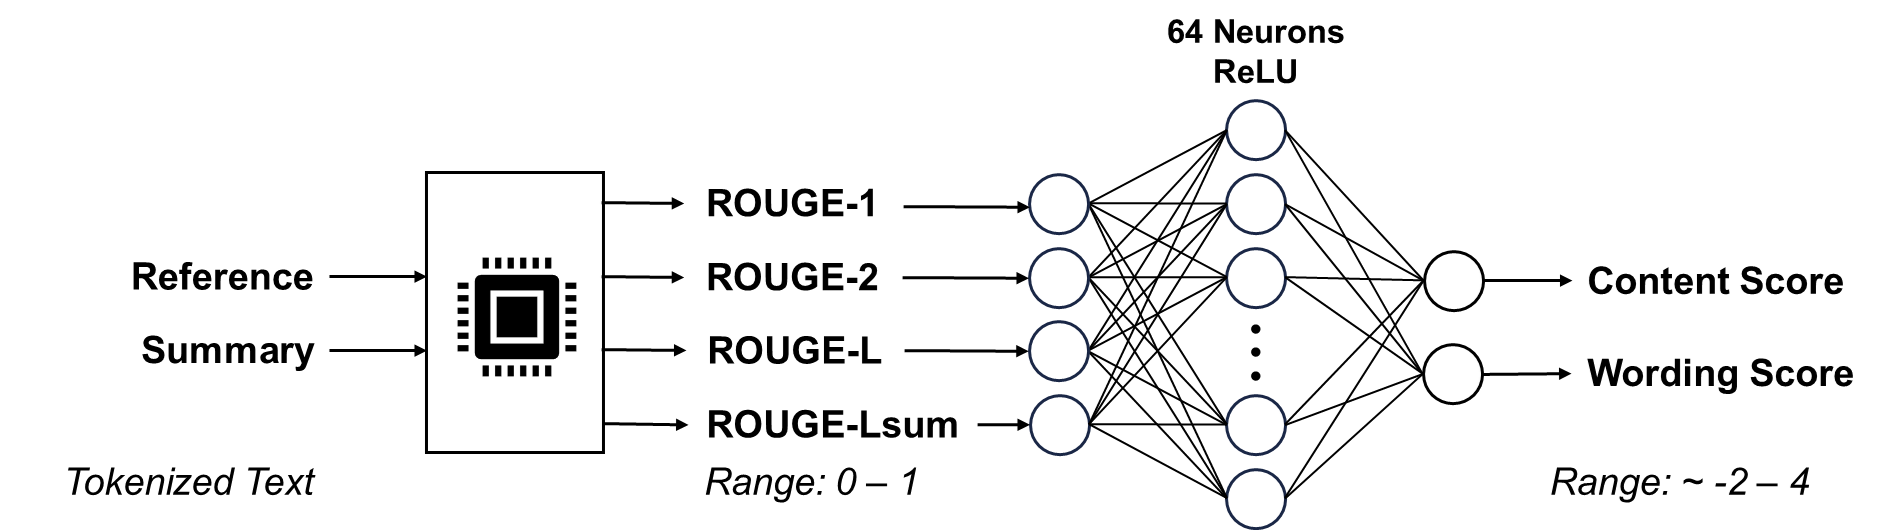
\includegraphics[keepaspectratio, width=\textwidth]{ROUGE-Based-Model.png}
\caption[ROUGE-Based Model Architecture]{Architecture of the ROUGE-Based Model.}
\label{fig:rouge-based-model}
\end{figure}

% \subsubsection{Hyperparameters}
% 
% \begin{itemize}
%     \item \textbf{Stopword Removal:} Determines whether stopwords are removed during processing.
%     \item \textbf{Stemming:} Controls whether stemming is applied to reduce words to their root form.
%     \item \textbf{Lemmatization:} Controls whether lemmatization is used to obtain the base form of words.
%     \item \textbf{ROUGE metrics:} Specifies what combination ROUGE metrics are used..
%     \item \textbf{Hidden-dim:} Sets the number of hidden layers in the neural network.
%     \item \textbf{Hidden-layers:} Determines the number of hidden layers in the neural network.
%     \item \textbf{Activation function:} Specifies the activation function applied in the neural network.
%     \item \textbf{Learning rate:} Learning Rate.
%     \item \textbf{Epochs:} Determines the number of times the entire training dataset is passed through the neural network.
% \end{itemize}

\subsubsection{Hyperparameter Tuning}

During the development and training of the ROUGE-Based Model, various hyperparameters were explored and tuned using the Optuna\footnote{\href{https://optuna.org/}{Optuna - Website}} library. It was found, that removing stopwords and applying \gls{stemming} or \gls{lemmatization} had little to no impact on the models performance. Therefore stopwords were removed to reduce the number of \glspl{token} when calculating the \gls{rouge} scores and neither stemming nor lemmatization were applied, as they were unnecessary. For the models inputs, specific \gls{rouge} scores were used, including ROUGE-1, ROUGE-2, ROUGE-L, and ROUGE-Lsum. These scores were calculated using the Python library 'rouge-score'.\footnote{\href{https://pypi.org/project/rouge-score/}{rouge-score library - PyPI Website}}
It's worth noting that later in the project, another library called 'rouge-metric'\footnote{\href{https://pypi.org/project/rouge-metric/}{rouge-metric library - PyPI Website}}
was found, which could calculate the additional gls{rouge} scores. However, considering the likely marginal gains and to maintain consistency, it was decided not to re-implement the model with the new library.\\
Given the nature of this model and the task, where the network primarily maps the \gls{rouge} scores (ranging from 0 to 1) into the content and wording scores (ranging from -2 to 4), the \gls{nn} was quite robust against overfitting. Changes in the number of hidden neurons and \glspl{hidden-layer} (as log as there was at least one \gls{hidden-layer}) had minimal impact on performance. Notably, the selection of the \gls{activation function} played a bigger role; logistic functions like Sigmoid and tanh demonstrated poorer performance. However, ReLU and Leaky ReLU showed better results, ultimately leading to the adoption of ReLU in the final model.

\begin{itemize}
    \item \textbf{Stopword Removal:} Stopwords were removed.
    \item \textbf{\glsdisp{stemming}{Stemming} \& \glsdisp{lemmatization}{Lemmatization}:} Neither \gls{stemming} nor \gls{lemmatization} was used.
    \item \textbf{ROUGE Metrics:} \gls{rouge}-1, \gls{rouge}-2, \gls{rouge}-L, \gls{rouge}-Lsum
    \item \textbf{\glsdisp{hidden-layer}{Hidden-Layers}:} 1 Hidden Layer
    \item \textbf{\glsdisp{hidden-dim}{Hidden-Dim}:} 64 Neurons
    \item \textbf{\glsdisp{activation function}{Activation Function}:} ReLU
    \item \textbf{\glsdisp{lr}{Learning Rate}:} 0.01
    \item \textbf{\glsdisp{epoch}{Epochs}:} 10
\end{itemize}
%\begin{figure}[H]
%
\includegraphics[keepaspectratio]{placeholder.png}
%\caption{\textbf{\textit{Hyperparameter Importance Plot(s) - Placeholder Text}}}
%\label{fig:rouge-hyperparameter-importance}
%\end{figure}

\subsubsection{Training}
The models \gls{nn} is initialized with random weights. Before training, it is also given the mean length (number of characters) and the standard deviation in length of the summaries in the training set. These two additional values are used to normalize the lengths of summaries, when passing them to the network. Since there is no upper bound for how long a summary can be, Z-Score Normalization was applied: %$z=\frac{x-\mu}{\sigma}$
\begin{equation}\label{eq:z-score}
    z=\frac{x-\mu}{\sigma}
\end{equation}
\myequations{Z-Score Normalization}
Where $z$ is the normalized length $x$ of a summary. $\mu$ is the mean length of the summaries in the trainings set and $\sigma$ the standard deviation.\\
Since the \gls{rouge} metrics have no learnable parameters, the python library 'rouge-score' can be used to precalculate these scores prior to training.
These precalculated scores are used as inputs to train the network, using the \gls{mse} loss function over 10 training \glspl{epoch}.

\subsubsection{Limitations}
It's important to note that this model only receives the summary and the reference text the summary was based on. It does not consider the specific task asked of the students. In cases where the prompt asks for specifics on one part of the text, a summary focusing on that prompt may be evaluated as worse than a summary that stays more general.\\
The model also doesn't know what words were used, only whether they overlap with the reference. Therefore, it cannot determine whether objective and neutral language was used or how well lexis and syntax was used. Due to these limitations it was expected, that this model performs better on the content score, and poorly on the wording score. (Also as evident by the correlation matrix; \hyperref[fig:rouge-correlation-matrix]{Figure~\ref{fig:rouge-correlation-matrix}}.)

\begin{figure}[h]
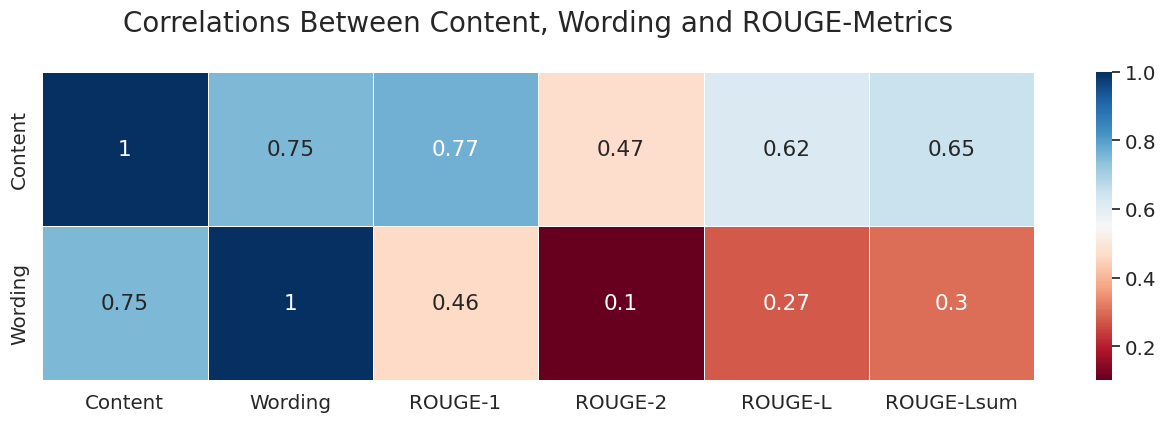
\includegraphics[keepaspectratio, width=\textwidth]{rouge_correlation_matrix.png}
\caption[ROUGE Metrics Correlation Matrix]{Correlations between Content and Wording scores and the used ROUGE Metrics}
\label{fig:rouge-correlation-matrix}
\end{figure}
